% Options for packages loaded elsewhere
\PassOptionsToPackage{unicode}{hyperref}
\PassOptionsToPackage{hyphens}{url}
%
\documentclass[
  12pt,
]{article}
\usepackage{lmodern}
\usepackage{amssymb,amsmath}
\usepackage{ifxetex,ifluatex}
\ifnum 0\ifxetex 1\fi\ifluatex 1\fi=0 % if pdftex
  \usepackage[T1]{fontenc}
  \usepackage[utf8]{inputenc}
  \usepackage{textcomp} % provide euro and other symbols
\else % if luatex or xetex
  \usepackage{unicode-math}
  \defaultfontfeatures{Scale=MatchLowercase}
  \defaultfontfeatures[\rmfamily]{Ligatures=TeX,Scale=1}
\fi
% Use upquote if available, for straight quotes in verbatim environments
\IfFileExists{upquote.sty}{\usepackage{upquote}}{}
\IfFileExists{microtype.sty}{% use microtype if available
  \usepackage[]{microtype}
  \UseMicrotypeSet[protrusion]{basicmath} % disable protrusion for tt fonts
}{}
\makeatletter
\@ifundefined{KOMAClassName}{% if non-KOMA class
  \IfFileExists{parskip.sty}{%
    \usepackage{parskip}
  }{% else
    \setlength{\parindent}{0pt}
    \setlength{\parskip}{6pt plus 2pt minus 1pt}}
}{% if KOMA class
  \KOMAoptions{parskip=half}}
\makeatother
\usepackage{xcolor}
\IfFileExists{xurl.sty}{\usepackage{xurl}}{} % add URL line breaks if available
\IfFileExists{bookmark.sty}{\usepackage{bookmark}}{\usepackage{hyperref}}
\hypersetup{
  hidelinks,
  pdfcreator={LaTeX via pandoc}}
\urlstyle{same} % disable monospaced font for URLs
\usepackage[margin=0.5in]{geometry}
\usepackage{graphicx}
\makeatletter
\def\maxwidth{\ifdim\Gin@nat@width>\linewidth\linewidth\else\Gin@nat@width\fi}
\def\maxheight{\ifdim\Gin@nat@height>\textheight\textheight\else\Gin@nat@height\fi}
\makeatother
% Scale images if necessary, so that they will not overflow the page
% margins by default, and it is still possible to overwrite the defaults
% using explicit options in \includegraphics[width, height, ...]{}
\setkeys{Gin}{width=\maxwidth,height=\maxheight,keepaspectratio}
% Set default figure placement to htbp
\makeatletter
\def\fps@figure{htbp}
\makeatother
\setlength{\emergencystretch}{3em} % prevent overfull lines
\providecommand{\tightlist}{%
  \setlength{\itemsep}{0pt}\setlength{\parskip}{0pt}}
\setcounter{secnumdepth}{-\maxdimen} % remove section numbering
\usepackage{setspace} \singlespacing

\usepackage{times} %set font to Times New Roman 

\usepackage{mathptmx} %set math font to match

%\usepackage[super,sort,compress]{natbib} %use sorted superscripts for references and compress runs of numbers
\usepackage[sort,compress]{natbib} %use sorted superscripts for references and compress runs of numbers

%\renewcommand{\bibname}{{REFERENCES CITED}}

\renewcommand{\bibsection}{\subsection*{REFERENCES CITED}} %rename references section to match requirements

\pagestyle{empty} %%delete the number at the bottom of the page

\bibliographystyle{unsrt}
\ifluatex
  \usepackage{selnolig}  % disable illegal ligatures
\fi

\author{}
\date{\vspace{-2.5em}}

\begin{document}

\textbf{PROJECT NARRATIVE}

\textbf{A. Background and Rationale}

The \textbf{goal} of this proposal is to map genetic modifiers of
tuberous sclerosis complex (TSC) outcomes in a genetically diverse mouse
population (Fig. \ref{fig:overview}). TSC is a rare autosomal dominant
disease caused by loss-of-function (LoF) mutations in either of the
genes \textit{TSC1} or \textit{TSC2} (\textit{TSC1/2}). These mutations
cause aberrant up-regulation of mammalian target of rapamycin (mTOR)
signaling, resulting in high rates of epilepsy, autism spectrum disorder
(ASD), and tumor formation in multiple organ systems \cite{17005952}.
However, presentation of TSC in the patient population is highly
heterogeneous ranging from subclinical to severe
\cite{gomez_tuberous_1999, 8423606, 17005952, 8057044, 29687738, 28127866, 29926239}.
There are at least three distinct contributors to this phenotypic
complexity: 1) a patient's specific TSC gene mutation; 2) the random
occurrence of somatic second-hit \textit{TSC1/2} mutations, and 3)
genetic modifiers, i.e., alleles inherited separately from the
\textit{TSC1/2} genes that alter the severity of TSC-associated
phenotypes. The \textbf{central hypothesis} of this project is that
genetic modifiers are a major source of patient heterogeneity. Despite
high heterogeneity within affected families sharing the same mutation
\cite{29687738, 28127866, 29926239}, TSC outcomes are more similar in
identical twins and within families than across families
\cite{18174550}, supporting the existence of genetic modifiers in the
human population.

\begin{figure}[ht!]
\includegraphics[width=\textwidth]{Fig1.png} 
\caption{\textbf{Project overview.} Breeding schematics show generation of A) DO-\textit{Tsc1} and B) DO-\textit{Tsc2} mice by crossing a DO female to an inbred mouse carrying a \textit{Tsc1} or \textit{Tsc2} null allele. DO-\textit{Tsc1} and DO-\textit{Tsc2} mice will be used in both aims of this proposal. Both mouse subpopulations will be run through all phenotyping pipelines and will have brain, kidneys, lung, liver, and heart harvested. RNA sequencing will be performed in brain for the DO-\textit{Tsc1} subpopulation and kidney for the DO-\textit{Tsc2} subpopulation. We will use AI technology to quantify C) seizures and D) histological phenotypes in all mice. We will map TSC-related phenotypic outcomes to E) individual QTL and F) to genetic interaction networks. G) Gene expression will be used as a mediator of genetic effects on phenotypes to identify molecular pathways influencing tumor and neurological outcomes.
}
\label{fig:overview}
\end{figure}

The \textbf{rationale} for this study is that by mapping genetic
modifiers, we will identify novel genes and pathways that can be
therapeutically targeted to mitigate poor outcomes. Although current
therapies that directly target mTOR signaling show promise in treating
TSC-associated conditions \cite{30760308, 29438097, 15578690, 20235887},
significant challenges remain. Indeed, some TSC tumors are unaffected by
treatment with rapamycin
\cite{15557109, 20235887, 25347447, 24395886, 22457331}, and both
seizures \cite{30305233} and tumors \cite{36028490, 22788941} develop
resistance to these therapies with long-term treatment. Thus, the
identification of alternative or adjunct therapies for TSC is critical
for long-term disease management. Previous work supports strategies
targeting mTOR-independent pathways. For example, genetic studies in
patients with TSC led to work in a mouse model demonstrating that
treatment with IFN-\(\gamma\) in combination with rapamycin was more
effective in reducing tumor growth and improving survival more than
rapamycin alone \cite{16845661}. Identification of this and other
alternative pathways \cite{15150271, 16803888, 24395886, 23715154}
through genetic modifier screens, may be critical for treatment of
refractory TSC.

Our preliminary data and prior reports definitively demonstrate the
existence of genetic modifiers of both neurological and tumor outcomes
in haploinsufficiency mouse models of TSC, providing a tractable
experimental platform for genetic discovery. Here, we propose to use
natural genetic variation in a population-based model of TSC to identify
additional molecular pathways that drive variation in TSC outcomes.

\begin{figure}[ht!]
\includegraphics[width=0.8\textwidth]{Fig2.png} 
\caption{\textbf{Previous experiments demonstrated that genetic background modifies seizure outcomes in a haploinsufficiency mouse model of TSC.} A) Breeding schematic describing generation of \textit{Tsc1}$^{+/-}$ mice on three different genetic backgrounds (B6, D2, and BXD87). B) Diagram and image of wireless EEG setup for seizure monitoring. C) Of all mice tested only female BXD87-HET- mice experienced seizures. D) Seizure counts for individual female BXD87-HET mice. E) Example EEG trace showing electrographic evidence of a seizure in a BXD87-HET mouse. All seizures were confirmed with concurrent video.
}
\label{fig:bxd}
\end{figure}

\textit{\underline{Genetic modifiers of seizure outcomes exist in a haploinsufficiency mouse model of TSC}}.
In \textbf{Aim 1} we will genetically map modifiers of neurological
outcomes in a mouse population model of \textit{Tsc1/2}
haploinsufficiency. Our recently completed study (DOD TS180087) tested
whether epilepsy outcomes in \textit{Tsc1}\(^{+/-}\) mice were
influenced by genetic background (Fig. \ref{fig:bxd}). We crossed a
C57BL/6J-\textit{Tsc1}\(^{+/-}\) mouse to multiple wild-type genetic
backgrounds--C57BL/6J (B6), DBA/2J (D2), and BXD87/Rww (BXD87)--allowing
us to test the relationship between strain background and disease
outcomes (Fig. \ref{fig:bxd}A). The BXD87 strain is a recombinant inbred
strain whose genome is a mosaic of the B6 and D2 genomes (Fig.
\ref{fig:bxd}A), which we chose because wild-type BXD87 mice are
outliers for both low hippocampal volume and poor cognitive performance
\cite{26449520, 28544613, 29457871}, suggesting a developmentally
susceptible state to poor TSC outcomes. Because the carrier parent was
heterozygous for the \textit{Tsc1} knockout, the F1 progeny could
inherit either one knockout allele (HET) or the B6 wild-type allele (WT)
(Fig. \ref{fig:bxd}A). We performed five-day video-electroencephalogram
(EEG) monitoring (starting around postnatal day 70) in N = 48 mice (Fig.
\ref{fig:bxd}B). We found that only BXD87-HET mice developed
spontaneous, tonic-clonic seizures when carrying a single copy of the
\textit{Tsc1} null allele. Over the course of our experiment 4 out of 7
BXD87 females had a total of 61 seizures (Fig. \ref{fig:bxd}C-D),
averaging 1.7 seizures per BXD87 female mouse per day. This is the first
time that a mouse model has been observed to develop chronic epilepsy
without an induced second hit to \textit{Tsc1/2}, demonstrating that a
single germline mutation of \textit{Tsc1} can cause chronic seizures in
mice in a manner that is modified by genetic background. We note that
haploinsufficiency models of spontaneous seizures have been reported
before; however, in these models early-life epilepsy resolved by
post-natal day 19 \cite{25081057}, well before adulthood, and hence does
not recapitulate the chronic epilepsy of the most severely affected
human patients. We can make two important observations about the
genetics of epilepsy in our BXD87-HET model. First, the appearance of
seizures in BXD87, but not the parent strains B6 and D2, implies that
there must be at least two genetic modifiers in BXD87 responsible for
epilepsy; If there were only one, we would have observed seizures in
either B6-HET or D2-HET mice. Second, we observed seizures only in
around half of the female BXD87-HET mice. Based on our cross design with
a B6-\textit{Tsc1}\(^{+/-}\) dam (Fig. \ref{fig:bxd}A), we infer that
one of the modifier alleles may be on the X chromosome and that
incomplete penetrance may be due to random X inactivation
\cite{15818384, 9618446}. We are currently testing this hypothesis,
which is out of the scope of this project. However, to maximize our
chance of detecting an X-linked modifier in this study, we will reverse
the cross so that the sire is the inbred carrier and the dam is the
genetically diverse, non-carrier. In this design, progeny of all sexes
will have genetic variation on the X chromosome.

Our data above demonstrate that the polygenic combination of variants
inherited by BXD87 from the B6 and D2 strains cannot suppress
TSC-associated epilepsy. Mapping these modifiers only three strains (B6,
D2, and BXD87) is impossible due to insufficient genetic resolution.
However, using existing data on the BXD mapping panel available in the
Mouse Phenome Database \citep{31696236}, we performed a re-analysis of
hippocampal volume and spatial memory performance phenotypes, for which
BXD87 is an outlier strain (low hippocampal volume, poor spatial memory
performance) \citep{26449520}. Briefly, we performed SNP association
mapping for each trait individually and combined them using a Bayesian
mixture model \citep{22396665} to identify SNPs explaining BXD87's
outlier status (Fig. \ref{fig:meta}). The top-ranked SNP overall was on
chromosome 4 and linked to the gene \textit{Gabbr2}. The human ortholog,
\textit{GABBR2}, has recently been implicated as a significant epilepsy
modifier gene in TSC (Farach et al., abstract to the International TSC
Research Conference 2021). The unlinked locus with the next most
significant SNP was on the X chromosome. The top SNP in this locus is
linked to the gene \textit{Ubqln2}, which encodes the protein Ubiquilin
2. Significantly, human Ubiquilin 2 has been shown to be an activator of
mTORC1 signaling \citep{26740621, 30804504}. This analysis strongly
suggests that: 1) genetic modifiers of baseline phenotypes in mice can
predispose strains to dramatically different TSC outcomes, and 2) mouse
modifier genes may translate directly to human TSC. While this analysis
is only suggestive, we will be able to validate the locations of TSC
modifier alleles and potential specific roles for \textit{Gabbr2} and
\textit{Ubqln2} through gene-expression and genetic mapping studies in
this proposal.

\begin{figure}[ht!]
\includegraphics[width=\textwidth]{Fig3.png} 
\caption{\textbf{Meta-analysis of outlier phenotypes in BXD87 mice} Using the Mouse Phenome Database, we re-analyzed neurological traits (hippocampal volume and radial arm maze performance) for which BXD87 is an outlier among all BXD strains. The top two loci were on chr 4 and chr X, and the top SNPs were linked to \textit{Gabbr2} and \textit{Ubqln2}, respectively. Both genes have a strongly plausible role in TSC-associated epilepsy.}
\label{fig:meta}
\end{figure}

\textit{\underline{Genetic modifiers of tumor outcomes exist in haploinsufficiency mouse models of TSC.}}
In \textbf{Aim 2} we will genetically map modifiers of tumor outcomes in
a population model of \textit{Tsc1/2} haploinsufficiency. Unlike
epilepsy, there is substantial prior work in rodents showing that
genetic variation is an important driver of tumor outcomes in
\textit{Tsc1/2} haploinsufficiency \cite{20235887}. In Eker rats, which
carry a null allele of \textit{Tsc2}, variation in kidney tumor size and
number have been mapped to alleles on rat chromosomes 3 \cite{11735216}
and 5 \cite{14654943}. In mice carrying a null \textit{Tsc2} allele,
tumor number, extent, and location vary by strain background.
Specifically, A/J-\textit{Tsc2}\(^{+/-}\) mice had a substantially
higher burden of kidney tumors than 129S4/SvJae-\textit{Tsc2}\(^{+/-}\)
mice \cite{10491404}, while 129S4/SvJae-\textit{Tsc2}\(^{+/-}\) mice had
a higher burden of liver tumors compared to six other strains tested
\cite{20235887}. Similarly, a null allele of \textit{Tsc1} caused high
incidence of renal carcinoma with some lung metastases in BALB/c mice
compared to other strains, while the same allele caused early-life
mortality in one quarter of B6 pups \cite{15888477}. Together these
studies demonstrate that tumor outcomes in haploinsufficiency models of
TSC are highly heritable.

\textit{\underline{Rationale for a DO-TSC population model}}. The
heritability of TSC outcomes in inbred strains proves the existence of
modifier alleles, but does not identify them. Here we propose to map
these alleles using the Diversity Outbred (DO) mouse population. The DO
mice are a highly recombined, outbred population derived from eight
inbred founder strains \cite{22892839}, which capture 89\% of the known
genetic variation in laboratory mice \cite{17674098}. Three of the DO
founders--A/J, B6, and 129--have been shown to vary in TSC-related
clinical outcomes in the studies cited above. Additionally, while they
are not founder strains per se, nearly all variants in BALB/c and BXD87,
which also carry modifiers of TSC outcomes, are present in the DO
population. Thus, by generating F1 hybrids between carriers of
\textit{Tsc1/2} LoF mutations with DO mice (Fig. \ref{fig:overview}A-B),
we can model both the germline haploinsufficiency of many human patients
and the effects of background genetic diversity. We will make two
subpopulations, DO-\textit{Tsc1} with a B6-\textit{Tsc1}\(^{+/-}\) sire
(Fig. \ref{fig:overview}A) and DO-\textit{Tsc2} with an
A/J-\textit{Tsc2}\(^{+/-}\) sire (Fig. \ref{fig:overview}B). Given our
results above, the DO-\textit{Tsc1} population is nearly certain to have
significant variation in epilepsy outcomes, with both susceptible and
resistant mice. Likewise, given prior reports on tumors in
A/J-\textit{Tsc2}\(^{+/-}\) mice, the DO-\textit{Tsc2} population is
nearly certain to have significant variation in tumor outcomes. Thus,
these subpopulations separately have power to detect strong modifier
genes. However, because poor neurological and tumor outcomes often occur
in the same patient, we will phenotype both subpopulations for both
categories of outcome and perform pooled analyses for universal
modifiers of \textit{Tsc1/2} LoF. By pairing clinical phenotypes with
high-throughput molecular data, a strategy called systems genetics, we
can further identify the regulatory effects of modifier alleles on genes
and pathways that drive variation \cite{24296534}. Systems genetics in
the DO population is a widely adopted design
\cite{35277432, 33687326, 26614740, 27309819, 28916633, 30840070, 32467129, 32763908, 32795400, 32877673, 32917924, 33264334, 33619752, 34045313, 34324982, 34403447, 34653361, 34666007, 35383961, 35481286, 35616343, 35819478, 36028119, 36212994, 36649207, 36714272, 36788222, 36968078, 36993241, 37214876, 37082146, 37214980, 37276142, 37301941},
with highly mature software tools for genetic mapping \cite{30591514}
(Fig. \ref{fig:overview}E), gene network inference \cite{24204223} (Fig.
\ref{fig:overview}F), and gene expression mediation analysis
\cite{35533209}(Fig. \ref{fig:overview}G). We have successfully used DO
mice to map individual QTLs and infer genetic networks
\cite{28592500, 37217254} (Fig. \ref{fig:overview}E-F). Others have
successfully mapped tumor outcomes using modifier screens similar to
this proposal \cite{27916600, 32796024}. We have also thoroughly studied
the effects of population structure on mapping studies in this
population \cite{33892506}. This prior work combined with our strong
preliminary data demonstrate that the DO-TSC population will be a
singularly powerful genetic discovery resource for TSC.

\textit{\underline{Artificial intelligence (AI) approaches for scalable, automated phenotyping.}}
One of the persistent problems for genetic mapping has been the
requirement for high-throughput phenotyping at the scale of hundreds of
individuals. This has traditionally meant either simple summaries of
complex observations (e.g., case vs.~control) or surrogate biomarkers
that may not capture the complete phenotype. However, recent advances in
AI and machine learning have dramatically lowered the barriers to subtle
phenotyping at scale, including scoring days-long home-cage behavior
videos
\cite{30127430, 26687221, 30573820, 31570119, 29779950, 37091193, 34718812, 35021077, 33729153},
non-invasive seizure monitoring \cite{36841241}, and analyzing
whole-slide images of tissues \cite{35202643, 31308507} (Fig.
\ref{fig:overview}C-D). We have pioneered applications of AI-based image
analysis for quantitative trait genetics. In a study of the
\textit{Far2} gene, which alters kidney aging phenotypes
\cite{29652635}, we demonstrated that AI approaches could recapitulate
known kidney phenotypes and detect novel phenotypes using only genotype
as a training label \cite{31220455}. In an extension of this work,
Dr.~Mahoney has an active R01 on histological imaging genetics to
further develop these tools. Taken together, this prior work and our
feasibility data (described below) demonstrate that we can use AI models
to robustly score seizure, behavioral, and histopathological phenotypes
at scale, and genetically map AI outputs as biologically meaningful
traits. Thus, our innovative AI-based phenotyping pipeline overcomes one
of the primary technical limitations of genetic mapping.

\textbf{B. Hypothesis and Objective}

The \textbf{objective} of this project is to identify novel genetic
modifiers of TSC outcomes and identify the gene expression signatures
that mediate these effects. To achieve this, we will perform a systems
genetics analysis of a novel DO-TSC population model. We hypothesize
that: 1) DO-TSC mice will vary significantly in seizure, behavioral, and
tumor outcomes;2) each outcome will have modifiers mapping to specific
locations in the genome, and 3) we will identify significant modifier
pathways using gene-expression mediation analysis.

\textbf{C. Specific Aims}

\textbf{Aim 1: Identify genetic modifiers of epilepsy and TANDs in TSC}
by: a) mapping genetic modifiers of epilepsy and TANDs in our DO-TSC
model and b) performing mediation analysis with brain gene expression to
identify the causal pathways driving poor neurological outcomes.

\textbf{Aim 2: Identify genetic modifiers of tumors in TSC} by: a)
mapping genetic modifiers of tumor outcomes in brain, kidney, and lung
in our DO-TSC model and b) performing mediation analysis with kidney
gene expression to identify the causal pathways driving poor tumor
outcomes.

\textbf{D. Research Strategy and Feasibility}

\textbf{Aim 1: Identify genetic modifiers of epilepsy and TANDs in TSC}

\textbf{Experimental approach:}

\textit{\underline{Generation of experimental mice:}} We will generate
two subpopulations of DO-TSC mice, which we designate as
DO-\textit{Tsc1} and DO-\textit{Tsc2} (Fig. \ref{fig:overview}A-B). We
will phenotype both sub-populations in both aims (Fig.
\ref{fig:overview}C-D). Each mouse will be an F1 hybrid between a
genetically unique female DO mouse and a male inbred carrier mouse. Each
F1 hybrid will also be genetically unique, because of recombination of
the DO dam's chromosomes during meiosis. For the DO-\textit{Tsc1}
subpopulation, we will use B6-\textit{Tsc1}\(^{+/-}\) mice as the
carrier sire. We will generate these mice as in our preliminary data,
using a cross between our B6-\textit{Tsc1}fl/fl mouse line and the
CMV-Cre line, which expresses Cre recombinase at the germline, causing
germline heterozygosity of \textit{Tsc1} LoF. For the DO-\textit{Tsc2}
subpopulation, we will use A/J-\textit{Tsc2}\(^{+/-}\) mice as the
carrier sire. These mice are not commercially available, so the JAX
Genetic Engineering Technologies (GET) group will generate this line
\textit{de novo} using CRISPR/Cas9 to knock out exons 5 through 8 in the
A/J background, matching the construct used in prior reports
\cite{10491404, 20235887}. In both subpopulations, we will genotype all
pups for the TSC mutation before weaning using standard PCR and retain
pups with a \textit{Tsc1/2} mutation for phenotyping. We will also
maintain detailed records of litter sizes and \textit{Tsc1/2} mutation
frequency as an additional phenotype. TSC mutations can cause fetal
death in humans \cite{15731990, 28868251, 18236061}, and prenatal death
would result in a significant deviation from the expected 50\% frequency
of \textit{Tsc1/2} mutations among pups.

\textit{\underline{Seizure and behavior monitoring.}} For
high-throughput seizure and behavioral phenotyping, we will use a novel
home-cage behavior system developed by TLR Ventures. This home-cage
behavior system was developed in collaboration with the Digital In Vivo
Alliance (DIVA), a consortium that includes JAX and supports the
development of automated home-cage technologies. DIVA cages have two
cameras, one overhead and another at a side angle, that stream video
directly to cloud-based computing centers. Once data are in the cloud,
DIVA cage software automatically applies AI models to identify animal
position (segmentation), identify key points on the body (key point
detection), predict respiratory rate, and identify loss of righting
reflex (LORR) during seizures. These data are stored for further
processing in a cloud-based data science environment, and user-interface
tools allow researchers to review videos, define segments of interest,
and train models \textit{de novo}. Starting around postnatal day 70, we
will put up to three littermate DO-TSC mice into the DIVA cages for
three consecutive days of continuous monitoring to measure the frequency
and duration of seizures, as primary outcomes. We will also measure
frequencies and durations of abnormal behaviors, such as backflipping,
abnormal grooming, or other stereotypies that have been associated with
ASD, as secondary outcomes. We will manually review periods of high
predicted probability of LORR to confirm seizures and fine-tune the
seizure detection model using manual annotations. Similarly, we will
apply and fine-tune existing models to detect periods of highly
stereotyped behavior, abnormal grooming activity, and identify
backflipping
\cite{30127430, 26687221, 30573820, 31570119, 29779950, 37091193, 34718812, 35021077, 33729153}.

\textit{\underline{Tissue collection:}} At 14 months of age, we will
collect brain, kidney, lung, liver, and heart tissue from each DO-TSC
mouse. All tissues will be fixed with formalin and embedded in paraffin
(FFPE) for long-term storage. We will separate brains along the corpus
callosum and use one hemisphere for RNA sequencing and the other for
histology.

\textit{\underline{RNA sequencing:}} To identify the gene expression
signatures that mediate the effects of genetic modifiers on epilepsy and
TANDs, we will perform bulk gene expression of brain tissue. Gene
expression analysis of all mouse brains from this study is beyond the
scope of this project. Thus, we will focus on DO-\textit{Tsc1}, which
has a high probability of manifesting heterogeneous neurological
outcomes. We will deliver DO-\textit{Tsc1} brain samples to the JAX
Genome Technologies Service for 50 base pair, paired-end bulk RNA
sequencing. Fastq files will be delivered to our group for analysis. We
will perform read alignment and gene expression quantification using
custom, publicly available RNA-seq pipelines developed by JAX
Computational Sciences \cite{jax_github}. This pipeline performs read
trimming to remove sequencing barcodes, quantifies gene expression using
the RNA-Seq by Expectation Maximization (RSEM) algorithm
\cite{21816040}, and delivers sample- and batch-level summary and
quality-control statistics, including Picard alignment metrics
\cite{picard} and a MultiQC \cite{27312411} report. Gene expression
levels will be normalized using a variance-stabilizing transformation
\cite{25516281, 23497356} for downstream processing.

\textit{\underline{Genotyping and reconstruction of ancestral haplotypes:}}
For background genotyping, we will use miniMUGA SNP genotyping arrays
\cite{33067325} to generate SNP-level genotypes for each mouse. We will
then compute the DO founder haplotypes using HaploQA \cite{haploQA}. We
will use haplotypes for genetic mapping \cite{25237114}.

\textit{\underline{Genetic mapping and power analyis:}} We will perform
two complementary forms of genetic mapping--linkage mapping and combined
analysis of pleiotropy and epistasis (CAPE)--each of which has unique
strengths. In linkage mapping, we correlate the haplotypes at individual
genetic markers with variation in quantitative traits, such as seizure
frequency. Linkage mapping seeks loci with strong marginal effects,
i.e., strong effects across many genetic backgrounds. We will perform
linkage mapping using R/qtl2 \cite{30591514} and define statistical
significance for QTLs using standard permutation-based statistical
thresholds \cite{8770605}. We will use sex and TSC-genotype as
interacting covariates to identify potential sex- and genotype-specific
modifiers. We will also use linear mixed models to account for the
effects of variable relatedness among individuals \cite{18385116}.
Because the DO mice are highly recombined, we expect that mapping in
this population will yield QTLs encompassing small genomic regions
(\(<\) 1 megabase (Mb)) with a small number of positional candidate
genes. With \(n = 400\) mice total, we will have 80\% power to detect
loci explaining 10\% of the variance in any individual phenotype
\cite{25237114}. This population size conforms to prior successful
mapping studies in DO-F1 hybrid mice \cite{27916600}. Because linkage
mapping is the most statistically stringent form of mapping, we have
powered our study for this analysis. Using gene expression from RNA
sequencing, we will also perform expression QTL (eQTL) analysis to
identify genetic loci regulating gene expression levels. We will map
eQTLs exactly as described above, once for each transcript. The effect
sizes for eQTLs are generally much more significant than QTLs for
clinical traits due to strong cis-regualtory effects. Thus, with
\(n=200\) mice with gene expression, we expect large numbers of eQTLs.
By identifying loci that influence both gene expression and traits, we
can more easily link trait variation to molecular mechanisms
\cite{29567659}. In addition to mapping to individual QTLs, we will use
CAPE, developed by Dr.~Tyler \cite{24204223}, to map trait variation to
epistatically interacting QTLs (genetic network inference). No gene acts
in isolation, and many genetic modifiers of TSC may depend on
interactions with the rest of the genome. CAPE leverages information
across multiple traits to infer directed epistatic interactions
affecting all traits simultaneously. The simultaneous analysis of
multiple traits increases power to detect QTLs over classical linkage
mapping \cite{28592500}. Moreover, CAPE allows inference of directed
interactions indicating which variant acts upstream of another variant
in an interacting pair, thereby aiding in interpretation of the
interaction and prioritization of causal positional candidate genes
\cite{26828925, 31694854}. Furthermore, the interactions identified are
consistent across all analyzed traits, allowing us to relate clinical
traits to genetic interactions through endophenotypes, such as the
expression of genes in the mTOR signaling pathway, which we will include
as traits in the analysis \cite{26828925, 28592500, 24297548}. As with
linkage mapping, we will use sex and TSC-genotype as interactive
covariates to ascertain sex- and genotype-specific effects. We will also
use linear mixed models to account for interindividual relatedness
\cite{33892506} and perform permutation testing to assess interaction
significance \cite{8770605}. We have experience using CAPE to analyze
seizure outcomes in mouse models of absence epilepsy \cite{25251056},
and complex traits in a DO population \cite{28592500} comparable to the
one proposed here. We expect that in this population we will be able to
generate multiple testable molecular hypotheses about genetic variants
that influence multiple clinical outcomes simultaneously.

\textit{\underline{Transcriptomic mediation analysis:}} One limitation
to all forms of genetic mapping is that the effects of individual loci
must be large enough to detect statistically. However, there is now
extensive evidence that most complex traits are highly polygenic, and
this polygenic effect is mediated through changes in transcriptional
profiles \cite{28622505, 31051098}. Thus, as a complement to genetic
mapping per se, we will also use gene expression to identify the
transcriptomic profiles driving heritable variation in neurological
outcomes, independent of individual genomic loci. To do this, we will
perform high-dimensional mediation analysis \cite{28637279}, which is an
extension of canonical correlation analysis that, in our case, seeks a
transcriptomic signature that is simultaneously correlated with
underlying genetics and phenotypic outcomes. Formally, if G, T, and P,
represent our genotype, transcriptome, and phenotype data matrices, we
define composite genetic, transcriptomic, and phenotypic scores,
\(s_g = G \cdot l_g\), \(s_t = T \cdot l_t\), and \(s_p = P \cdot l_p\),
respectively, through matrix multiplication of the data matrices with
loading vectors lg, lt, and lp that define each variable's importance to
the corresponding score. Using the theory of causal graphical models
\cite{21218138, 22496633}, we maximize the likelihood function
\(L = -\log|S| - \mathrm{tr}(\Sigma S^{-1})\), where \(\Sigma\) is the
correlation matrix of the scores (\(s_g\), \(s_t\), and \(s_p\)), \(S\)
is the model-implied covariance matrix for the perfect mediation model,
and \(|.|\) and \(tr\) denote the determinant and trace of a matrix,
respectively \cite{bollen_structural_1989}. This model encodes the
causal flow of information from genotype, through transcription, to
phenotype. The outputs of this analysis are the optimal scores and
loadings that define the causal influence of genetic background on TSC
outcomes. We will rigorously define the significance of mediation by
permuting the transcriptomes relative to the genotypes and phenotypes to
generate a null distribution for the path coefficient from genotype to
phenotype. To identify the significant pathways in the transcriptomic
score, we will rank all individual transcripts by their loadings, lt,
and perform gene set enrichment analysis (GSEA) \cite{16199517}. In this
way, the transcript rankings are a powerful complement to genetic
mapping because they allow inference of the causal importance of genes
and pathways, even when background modifier effects are highly
polygenic.

\textbf{Feasibility:} As feasibility data for this proposal, we trained
an AI model \textit{de novo} to detect LORR in manually coded frames
from videos of 25 mice during pentylenetetrazole-induced seizures (Fig.
\ref{fig:LORR}A). The model achieved greater than 95\% accuracy
detecting LORR in testing data (Fig. \ref{fig:LORR}B). As an example
readout, the model computes a time-varying probability (Fig.
\ref{fig:LORR}C, blue trace) that predicts when the mouse has fallen
vs.~is upright. Time intervals with high predicted probability were
strongly correlated with expert annotations of LORR (Fig.
\ref{fig:LORR}C, pink boxes). These data demonstrate that the DIVA cages
can robustly detect and quantify seizures at scale. The DIVA cages also
compute animal segmentations and pose-estimation phenotypes from which
we can score standard home cage behaviors, such as grooming.

\begin{figure}[ht!]
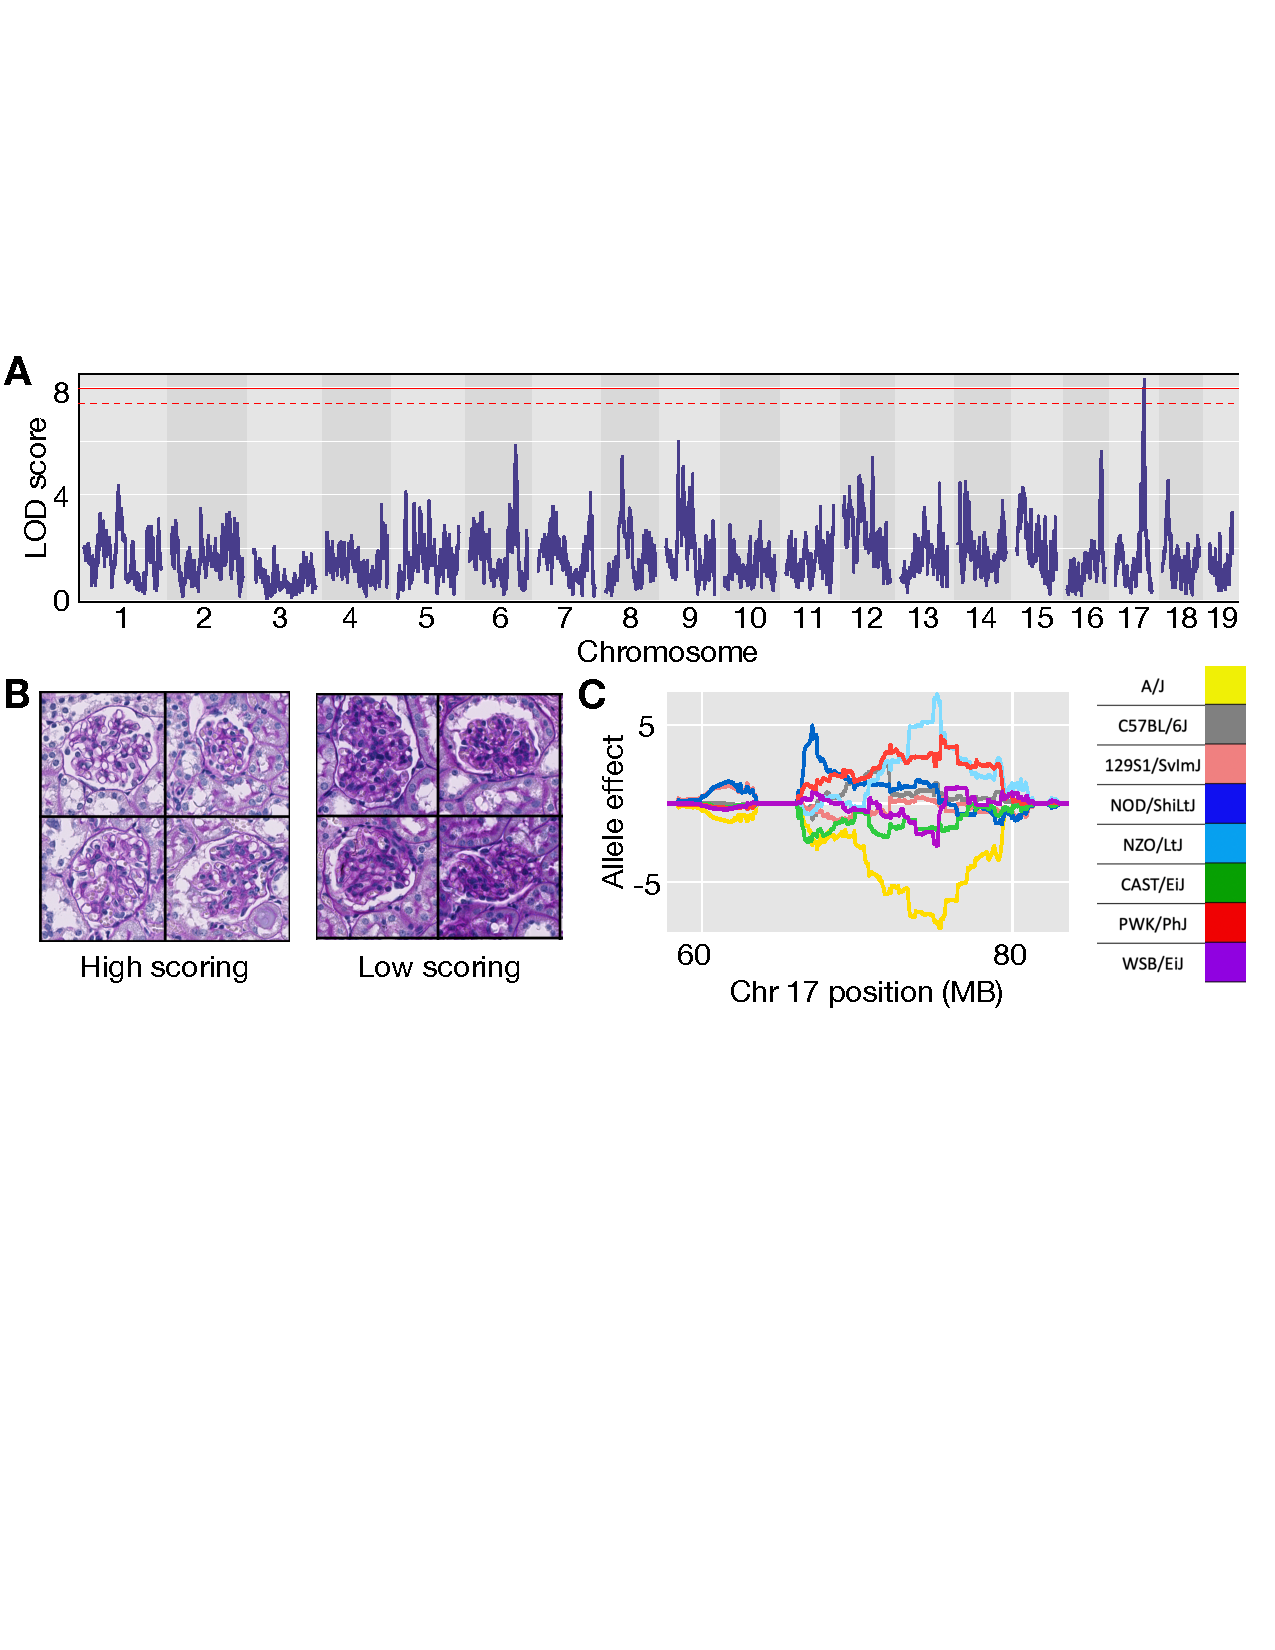
\includegraphics[width=\textwidth]{Fig4.png} 
\caption{\textbf{AI classification of seizures.} A) Still images of normal behavior (top row) and mice experiencing seizures (bottom row). The bottom row shows the loss-of-righting reflex (LORR) that is classified by the AI model as a seizure. B) Confusion matrix showing the counts of correct and incorrect classifications by the AI along with calculated accuracy, recall, and precision of the model. C) A time-varying probability of LORR predicted by the AI model at each frame of a video (blue trace). High probabilities indicate frames for which the AI predicted that the mouse had fallen over. Pink areas highlight frames for which an expert reviewer indicated that the mouse had fallen over.}
\label{fig:LORR}
\end{figure}

\textbf{Potential problems and alternative strategies:} We anticipate
three potential issues. First, we may not detect any QTLs at the
genome-wide significance level using any of the proposed strategies,
thereby limiting candidate gene prioritization from genetic mapping.
While we stress that our combined approach is designed to mitigate this
possibility, if it occurs, we anticipate that it will be due to both the
presence of a large number of modifiers and limited statistical power to
detect effects. If this transpires, we will use false discovery rate
(FDR) approaches \cite{24062767} to lower the burden of multiple testing
for our associations. We also note that high-dimensional mediation
analysis is an explicitly polygenic analysis that supports gene
prioritization independent of QTLs. Second, we may not have sufficient
genetic resolution to nominate candidate genes by mapping alone. While
current DO generations have linkage blocks that are substantially below
1 Mb, it is possible that our analyses may not resolve individual
candidate genes. If this transpires, we will pursue candidate gene
prioritization within QTLs using network-based approaches that Drs.
Mahoney and Tyler have extensively developed \cite{33889174, 31645420}.
Third, we may find that DO-TSC mice have heterogeneous seizure
presentations that are difficult to track with our existing AI tools.
Because we expect all animals having tonic-clonic seizures to have LORR,
we anticipate that thresholding the AI-generated probabilities at a low
level, e.g.~20\%, will guide us to epochs that are enriched for seizure
activity (see Fig. \ref{fig:LORR}). If we identify misclassified epochs,
we will first attempt to fine-tune the LORR model by manually annotating
a subset of these epochs as ground-truth labels. Barring that, following
Geschwind et al.~\cite{36841241}, we will perform unsupervised analyses
that cluster animal behaviors into groups, independent of annotations,
and manually annotate clusters corresponding to seizures and other
abnormal behaviors. In the worst case, we will review all videos in
their entirety, visually screening for seizures.

\textbf{Aim 2: Identify genetic modifiers of tumors in TSC.}

\textbf{Experimental approach:} For this aim we will use the same 400
DO-TSC mice developed in \textbf{Aim 1}. We will perform tissue
pre-processing, genotyping, genetic mapping, and mediation analysis
exactly as described above.

\textit{\underline{Histological imaging:}} We will deliver FFPE brain,
kidney, and lung tissue blocks to the JAX Histology Service for
sectioning and staining with hematoxylin and eosin (H\&E). Stained
slides will then be delivered to the JAX Microscopy Service for slide
scanning with a 40X objective. Whole-slide image files will be delivered
to our team for analysis. At the conclusion of this study, we will make
all histological images available to the public.

\textit{\underline{Image processing and genetic mapping:}} To generate
histological phenotypes at the scale required for genetic mapping, we
will use an AI-based computer vision approach to automatically score the
extent of tissue abnormalities without requiring extensive human
annotation. From each tissue image, we will extract tiles, or
sub-images, of 299x299 pixels, which we will input into the Inception v3
deep neural network \cite{inception}. The Inception v3 model is a
top-performing network for natural image classification
\cite{farooq2020advanced}. We will perform transfer learning
\cite{dutta2022multi}, where we remove the last layers of the model and
retain the numerical features at the second-to-last layer as a black-box
feature vector encoding histological image structure. This transfer
learning approach has been applied heavily in the cancer field with
remarkable success \cite{31010833, 32968067}. From the black-box feature
vector, we will perform principal components analysis (PCA) to identify
the dominant axes of variation across all images of the same tissue. For
each sample, we will average the PCA scores over tiles to compute
mouse-level scores, which we will map as quantitative traits, using the
techniques described in \textbf{Aim 1}. We will visualize the learned
tissue features from our model using example montages, where we compare
high- and low-scoring tiles to detect differences.

\textit{\underline{RNA sequencing and analysis:}} To identify the gene
expression signatures that mediate the effects of genetic modifiers on
tumors, we will perform bulk gene expression of kidney tissue. Gene
expression analysis of all mouse tissues from this study is beyond the
scope of this project. Thus, we will focus on DO-\textit{Tsc2} kidneys,
which have a high probability of manifesting heterogeneous tumor
outcomes.

\textit{\underline{Tissue biobanking:}} We will biobank the brain, lung,
and kidney tissue not used for histology or RNA sequencing, as well as
all liver and heart samples, from each DO-TSC mouse. We expect our
results from this project to provide a strong rationale to generate
comprehensive histological and gene expression data for these remaining
samples. We will also make the biobanked tissues available to the wider
TSC research community upon reasonable request.

\textbf{Feasibility:} In ongoing work for Dr.~Mahoney's R01, we have
analyzed kidney aging in a population of 500 DO mice using the strategy
described above (in preparation; Fig. \ref{fig:histo}). Using
whole-slide images of periodic acid-Schiff-stained kidney sections, we
extracted features from \textasciitilde150k individual glomeruli and
performed PCA to automatically identify age-related tissue features
across the population. We genetically mapped these AI-derived scores and
identified a significant QTL on chr. 17 (Fig. \ref{fig:histo}A).
Examples of high- and low-scoring glomeruli show marked differences in
mesangial matrix expansion, an age-associated histopathology (Fig.
\ref{fig:histo}B), and cellularity, both of which we have validated
quantitatively (data not shown). The allele effects for this AI-derived
trait show that inheriting the A/J allele leads to worse outcomes while
the NZO/LtJ allele leads to better outcomes (Fig. \ref{fig:histo}C). We
have nominated high-confidence candidate genes within this locus--Xdh
and Birc6--which have variants specific to the A/J and NZO/LtJ
backgrounds, respectively, and strong evidence for association to kidney
phenotypes \cite{23249873, 29795190}. We have ongoing experiments with
CRISPR knock-in mice to validate these effects. While this study does
not speak to the hypotheses of this project, it demonstrates feasibility
for mapping genetic modifiers of histological outcomes using AI-derived
traits.

\begin{figure}[ht!]
\includegraphics[width=0.8\textwidth]{Fig5.png} 
\caption{\textbf{Previous study demonstrating feasibility of mapping novel histological phenotypes generated by AI models.} A) QTL map for an age-related, AI-generated histological feature. This feature had a genome-wide significant QTL on mouse chromosome 17. The solid and dashed red lines indicate genome-wide significance of 1\% and 5\% respectively. B) Montage of images comparing glomeruli that scored high and low for this mapped feature. High- and low-scoring glomeruli differed in mesangial matrix expansion (darker purple staining) and cellularity (number of nuclei per glomerulus). C) Founder allele effects at the QTL for this feature. Each founder is represented by one color. NZO alleles (light blue) were associated with better outcomes than A/J alleles (yellow).}
\label{fig:histo}
\end{figure}

\textbf{Potential problems and alternative strategies:} We anticipate
two potential problems. First, bulk RNA sequencing of kidney tissues
necessarily mixes healthy tissue and tumor tissue, possibly limiting our
ability to detect causally important transcriptomic changes relative to
``passenger'' changes. We can detect this by performing mediation
analysis in reverse, with phenotypes as the mediator and gene expression
as the outcome. Individual transcripts that are highly ranked in both
models (i.e., with transcriptome as a mediator and an outcome) will be
considered confounded. If this occurs, we will cross-reference our
kidney expression to existing eQTL data from DO kidneys in mice without
a TSC insult \cite{33687326}. This will give added confidence in
specific, genetically encoded transcript changes that cannot be due to
tumor-composition effects. These data will also provide a strong
rationale for follow-up proposals to generate single-cell and spatial
transcriptomic atlases from our biobanked samples, from which we can
deconvolve our bulk expression computationally \cite{30670690}. A second
potential problem is that we may fail to detect overt lesions using an
unsupervised PCA approach. While we consider this extremely unlikely, if
this occurs, we anticipate that it will be due to the heterogeneity of
normal tissue structure in the DO obscuring the effects of relatively
rarer lesional tissue. If our PCA montages (see Fig. \ref{fig:histo}B)
do not contrast normal tissue with lesional tissue, then we will consult
with JAX's on-site veterinary pathologist to both annotate the learned,
non-lesional features and provide annotations of lesions that were
missed by our analysis. With ground-truth labels of novel features, we
can train models \textit{de novo} to detect such features directly,
which we will use as an additional phenotype. If lesions are extremely
rare, we will apply outlier detection methodologies
\cite{crammer_needle_2004} to identify image tiles that exist far
outside the distribution of healthy tissue. If all else fails, we will
review each whole-slide image in its entirety, manually annotating
abnormalities. These images will become public upon project completion
for researchers in the wider community to apply their expertise and
define novel phenotypes.

\textbf{Overall timeline}

Breeding of the DO-\textit{Tsc1}\(^{+/-}\) mice will begin immediately
and the first round of experimental mice will be available around three
months. Mice will be bred to generate waves of approximately 50 mice.
Home-cage behavior monitoring will occur continuously as new
experimental waves arrive. After home-cage monitoring monitoring, mice
will be housed until 14 months of age (17 months into the project), at
which time they will sacrificed for tissue harvest. In parallel with the
DO-\textit{Tsc1}\(^{+/-}\) experiment, we will generate the
A/J-\textit{Tsc2}\(^{+/-}\) model using CRISPR. The full CRISPR
pipeline, from generating the first knockouts and backcrossing to remove
off-target effects, will take approximately 9 months. We will then begin
breeding of the DO-\textit{Tsc2}\(^{+/-}\) mice, and experimental mice
will be available by the end of Year 1. Thus, the
DO-\textit{Tsc2}\(^{+/-}\) experiment will lag behind the
DO-\textit{Tsc1}\(^{+/-}\) and be complete at around 29 months into the
project. We will perform seizure and behavior analyses continuously
throughout the study, monitoring model performance and fine-tuning as
necessary. When all tissues from both subpopulations are collected, we
will generate histological data and perform RNA sequencing in a single
batch (around month 30). In the final 6 months, we will perform
histological image analysis and genetic mapping, draft manuscripts, and
prepare follow-up grant proposals.

\textbf{Integration of aims and project growth:} The aims of this
project are conceptually and operationally distinct, but form an
integrated whole. If both are successful, we will be positioned to
perform a joint analysis of neurological and tumor outcomes. Indeed, we
anticipate that many genetic modifiers will be pleiotropic across both
classes of outcomes \cite{28592500}. By mapping pleiotropic modifiers,
we may identify universal disease-modifying targets. Going forward, we
believe that the DO-TSC model from this Idea Development proposal will
provide a platform for multiple, critical follow-up research programs,
including an extended search for disease modifiers, pharmacogenetic
studies of resistance to therapies (\textit{e.g.}, rapalogs), and
pre-clinical drug screening in genetically diverse animals, minimizing
the probability of false-positive hits. Thus, by developing the DO-TSC
population model, we will enable a significant new paradigm for model
systems studies of TSC.

\pagebreak

\bibliography{pmid_refs.bib}

\end{document}
